\section{Kiến trúc hệ thống}
Hệ thống được thiết kế với hai module với chức năng của từng module được mô tả dưới đây:
\begin{itemize}
    \item \textbf{Module thu thập dữ liệu cử chỉ:} Đầu vào của khối này là dữ liệu cử chỉ được thu thạp từ các cảm biến uốn cong và cảm biến gia tốc. Dẽ liệu sau khi thu thập sẽ được đóng goi và gửi về module nhận dạng cử chỉ.
    \item \textbf{Module nhận dạng cử chỉ} Dữ liệu được gửi về từ module thu thập sẽ được xử lý, phân loại và đình hình lại dữ liệu để đưa vào mô hình LSTM. Đầu ra của mô hình LSTM sẽ là kết quả dự đoán cử chỉ dưới dạng văn bản và sẽ được chuyển đổi thành giọng nói qua khối Text-to-speech.
    \item \textbf{Module chuyển văn bản thành giọng nói}: Khi nhận được output đầu ra, module này có chức năng chuyển đầu ra từ dạng one-hot-code output sang dạng văn bản, từ văn bản đó sử dụng thư viện pyttsx3 để phát ra âm thanh như mong muốn đã được cấu hình trước đó trong file config
\end{itemize}
\begin{figure}[H]
    \centering
    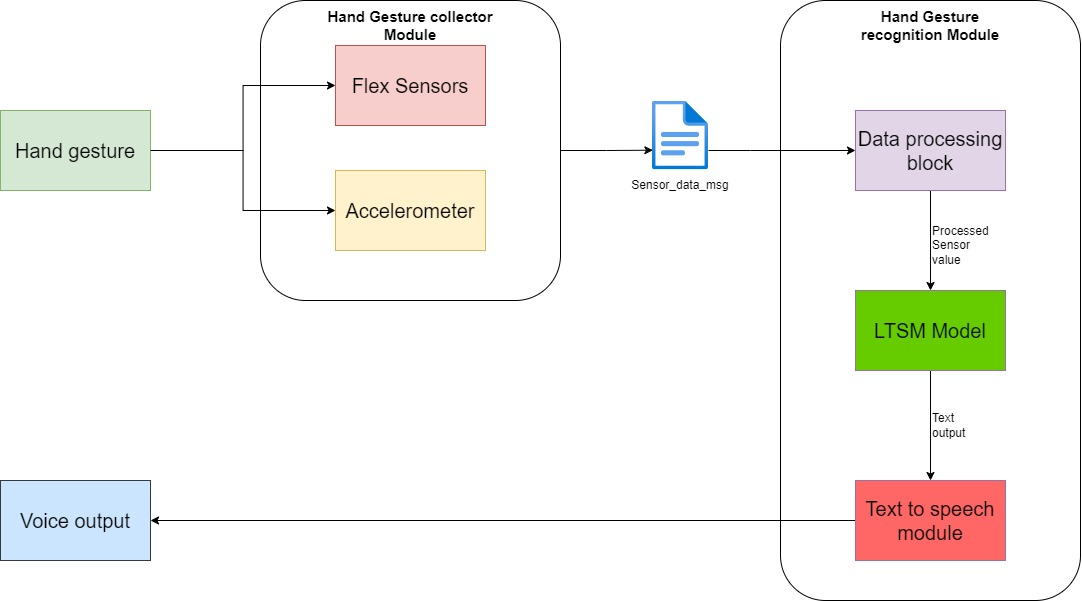
\includegraphics[width=\textwidth,height=\textheight,keepaspectratio]{Images/Theoretical basis/FlexArchitecture.jpg}
    \caption{Kiến trúc tổng quan của hệ thống}
    \label{fig:enter-label}
\end{figure}
\textbf{Mô tả luồng dữ liệu }
\textbf{Hand Gesture} (Cử chỉ tay): Cử chỉ tay là đầu vào của hệ thống. Các cảm biến uốn cong và gia tốc kế trong mô-đun thu thập cử chỉ tay sẽ ghi nhận và gửi dữ liệu này đến khối xử lý dữ liệu.\

\textbf{Sensor Data Message }(Thông điệp dữ liệu cảm biến): Dữ liệu từ cảm biến được đóng gói thành thông điệp và truyền tới mô-đun nhận diện cử chỉ tay.\

\textbf{Processed Sensor Value} (Giá trị cảm biến đã xử lý): Dữ liệu cảm biến được xử lý trong khối xử lý dữ liệu và các đặc trưng được trích xuất.\

\textbf{Text Output} (Đầu ra văn bản): Mô hình LSTM dự đoán cử chỉ tay và chuyển đổi nó thành văn bản.\

\textbf{Voice Output} (Đầu ra giọng nói): Văn bản từ mô hình LSTM được chuyển đổi thành giọng nói và phát ra ngoài thông qua mô-đun chuyển văn bản thành giọng nói.\


Hệ thống này bao gồm hai mô-đun chính và một module phụ: một mô-đun thu thập cử chỉ tay, một mô-đun nhận diện cử chỉ tay và module phát âm thanh. Mô-đun thu thập cử chỉ tay sử dụng các cảm biến uốn cong và gia tốc kế để ghi nhận dữ liệu cử chỉ tay, sau đó truyền dữ liệu này đến mô-đun nhận diện cử chỉ tay. Tại đây, dữ liệu cảm biến được xử lý và đưa vào mô hình LSTM để dự đoán cử chỉ tay dưới dạng văn bản. Cuối cùng, văn bản này được chuyển đổi thành giọng nói dựa trên module phát âm thanh


\subsection{Module thu thập dữ liệu cử chỉ}
\begin{figure}[H]
    \centering
    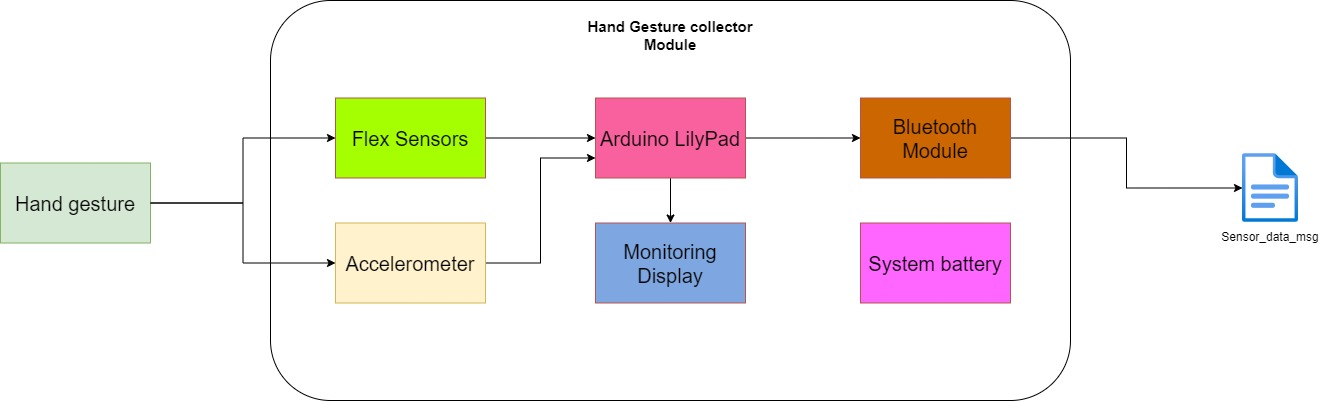
\includegraphics[width=\textwidth,height=\textheight,keepaspectratio]{Images/Theoretical basis/HandGestureCollector.jpg}
    \caption{Kiến trúc module thu thập dữ liệu cử chỉ}
    \label{fig:enter-label}
\end{figure}

Sơ đồ mô tả một hệ thống thu thập cử chỉ tay, gồm các thành phần sau:
\begin{itemize}
\item 1. Hand gesture (Cử chỉ tay): Đây là đầu vào của hệ thống, là các cử chỉ tay cần được nhận diện.
\item 2. Flex Sensors (Cảm biến uốn cong): Nhận tín hiệu từ cử chỉ tay và chuyển tiếp đến Arduino LilyPad.
\item 3. Accelerometer (Gia tốc kế): Cũng nhận tín hiệu từ cử chỉ tay và chuyển tiếp đến Arduino LilyPad.
\item 4. Arduino LilyPad: Xử lý dữ liệu nhận được từ Flex Sensors và Accelerometer. Sau đó, chuyển tiếp dữ liệu này đến các thành phần khác.
\item 5. Monitoring Display (Màn hình giám sát): Hiển thị dữ liệu và thông tin từ Arduino LilyPad để người dùng có thể theo dõi.
\item 6. Bluetooth Module (Mô-đun Bluetooth): Truyền dữ liệu từ Arduino LilyPad tới file data
\item 7. System Battery (Pin hệ thống): Cung cấp năng lượng cho toàn bộ hệ thống.
\end{itemize}


Dữ liệu được thu thập từ cử chỉ tay sẽ được xử lý và truyền đi qua mô-đun Bluetooth, sau đó lưu vào file data
\subsection{Module nhận dạng cử chỉ}
\begin{figure}[H]
    \centering
    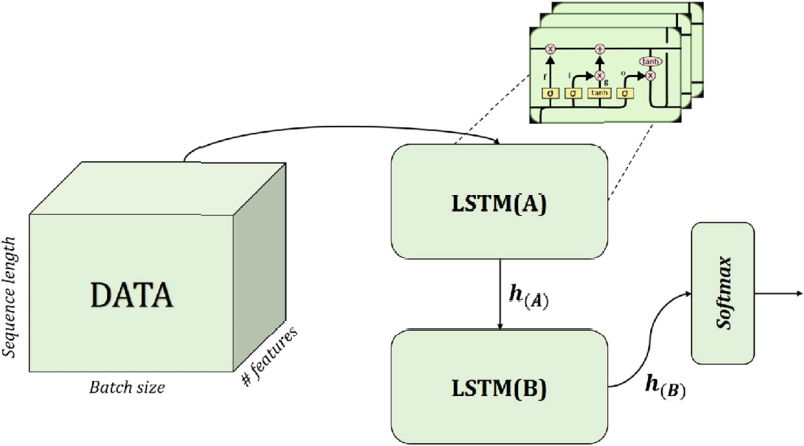
\includegraphics[width=\textwidth,height=\textheight,keepaspectratio]{Images/Theoretical basis/lstm model.png}
    \caption{Kiến trúc model dự đoán cử chỉ}
    \label{fig:enter-label}
\end{figure}

Sơ đồ mô tả một mô hình học sâu sử dụng LSTM (Long Short-Term Memory) để dự đoán xác suất của các hành động, như mua hoặc bán. Dưới đây là mô tả chi tiết của từng thành phần trong mô hình:
\begin{itemize}
     

\item 1. DATA (Dữ liệu):\\
   - Đầu vào của mô hình là một khối dữ liệu ba chiều với các thông số:\\
     - Sequence length: Độ dài chuỗi thời gian của dữ liệu.\\
     - Batch size: Kích thước lô, số lượng chuỗi thời gian trong một lô.\\
     - Features: Số lượng đặc trưng trong mỗi bước thời gian của chuỗi.

\item 2. LSTM(A):\\
   - Dữ liệu đầu vào được đưa vào lớp LSTM đầu tiên, gọi là LSTM(A). LSTM là một loại mạng nơ-ron hồi tiếp được thiết kế để xử lý và dự đoán các chuỗi dữ liệu thời gian.

\item 3. h(A):\\
   - Đầu ra của LSTM(A) là một vector ẩn (hidden vector), ký hiệu là h(A). Vector này lưu trữ thông tin trạng thái ẩn của LSTM sau khi xử lý dữ liệu đầu vào.

\item 4. LSTM(B):\\
   - Vector ẩn h(A) sau đó được đưa vào một lớp LSTM thứ hai, gọi là LSTM(B). Lớp này tiếp tục xử lý dữ liệu và tạo ra một vector ẩn mới, ký hiệu là h(B).

\item 5. h(B):\\
   - Đầu ra của LSTM(B) là vector ẩn h(B), lưu trữ thông tin trạng thái ẩn sau khi dữ liệu được xử lý qua hai lớp LSTM.

\item 6. Softmax:\\
   - Vector ẩn h(B) được đưa vào một lớp Softmax. Lớp này chuyển đổi vector thành các xác suất để dự đoán các hành động cụ thể.

\item 7. Output:\\
   - Đầu ra cuối cùng của mô hình là các xác suất được tạo ra bởi lớp Softmax, ví dụ như label 0,1,2 được mã hóa dưới dạng one-hot-code

\end{itemize}
Mô hình này có thể được sử dụng cho các ứng dụng như dự đoán thị trường chứng khoán hoặc các bài toán khác liên quan đến chuỗi thời gian, nơi việc xác định các hành động dựa trên dữ liệu lịch sử là quan trọng. Sơ đồ này minh họa cách dữ liệu được xử lý qua các lớp LSTM và sau đó chuyển đổi thành các xác suất đầu ra thông qua lớp Softmax.


\subsection{Module phát âm thanh}
\begin{figure}[H]
    \centering
    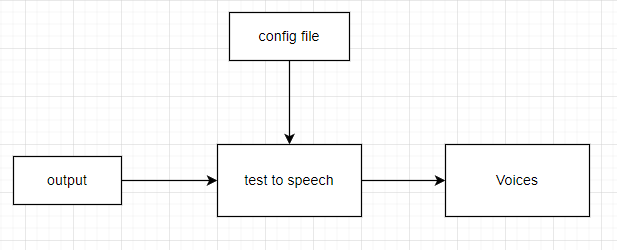
\includegraphics[width=\textwidth,height=\textheight,keepaspectratio]{Images/Theoretical basis/test2speech.png}
    \caption{Kiến trúc module chuyển đầu ra dự đoán thành giọng nói}
    \label{fig:enter-label}
\end{figure}

Sơ đồ mô tả module phát âm thanh sau khi dự đoán đúng một hành động sử dụng thư viện text-to-speech pyttsx3

Thư viện pyttsx3 cung cấp một giao diện đơn giản và nhất quán cho việc chuyển đổi văn bản thành giọng nói trên nhiều nền tảng. Kiến trúc của nó được thiết kế để trừu tượng hóa các chi tiết đặc thù của nền tảng, cho phép các nhà phát triển tập trung vào chức năng TTS ở mức cao. Các thành phần cốt lõi bao gồm bộ máy, trình điều khiển và cơ chế cấu hình, hoạt động cùng nhau để cung cấp tổng hợp giọng nói liền mạch và tùy chỉnh. Thiết kế của thư viện đảm bảo tính tương thích, linh hoạt và dễ sử dụng, biến nó thành công cụ mạnh mẽ để thêm khả năng TTS vào các ứng dụng Python.

Cụ thể âm thanh được phát ra khi có một output chỉ index trong file config giọng nói trước đó có sẵn, kiến trúc này sẽ lấy chính xác vị trí âm thanh giọng nói phát ra như mong muốn.